In order to calculate the color score the \textit{Quantification of Color}\cite{Fernandez_Alcon_2009} algorithm was implemented in which the distance of each pixel to a defined set of colors is evaluated.

The original image is first filtered using a low pass Gaussian filter in order to reduce noise. Then for for each pixel with the lesion area the euclidean distance from 6 RGB values is calculated. The 6 RGB values, as shown in table \ref{fig:tds_color}, represent the colors that are relevent to the TDS calculation.

\begin{table}[H]
\centering
\small
    \begin{tabular}{ | l | l | l | l |}
    \hline
    Color & R & G & B \\ \hline
    White & 255 & 255 & 255 \\
    Red & 204 & 51 & 51 \\
    Light Brown & 153 & 102 & 0 \\
    Dark Brown & 51 & 0 & 0 \\
    Blue Gray & 51 & 153 & 255 \\
    Black & 0 & 0 & 0 \\ \hline

    \end{tabular}

    \caption{RGB values of the six possible TDS-relevent colors\cite{Fernandez_Alcon_2009}}
    \label{fig:tds_color}

\end{table}

For each color a counter is incremented when a pixel is found that is closest to it. The end results are divided by the total number of pixels within the lesion's boundaries. For each color with a value greater than 0.01 a point is given to the TDS C score.

\begin{figure}[H]
    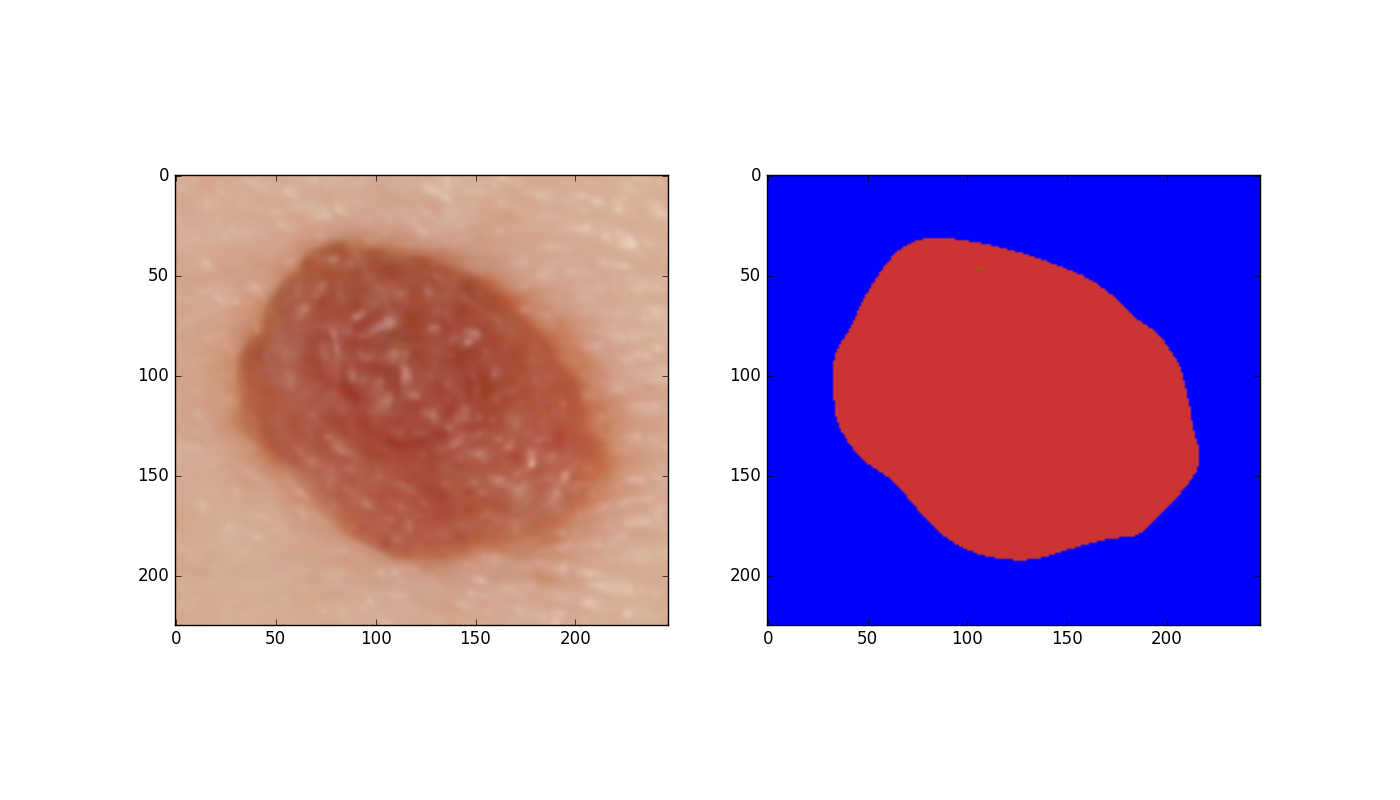
\includegraphics[height=8cm,keepaspectratio]{assets/color/examples/color_1.png}
    \caption{Example of color score 1}
    \label{fig:color_1}
\end{figure}
\begin{figure}[H]
    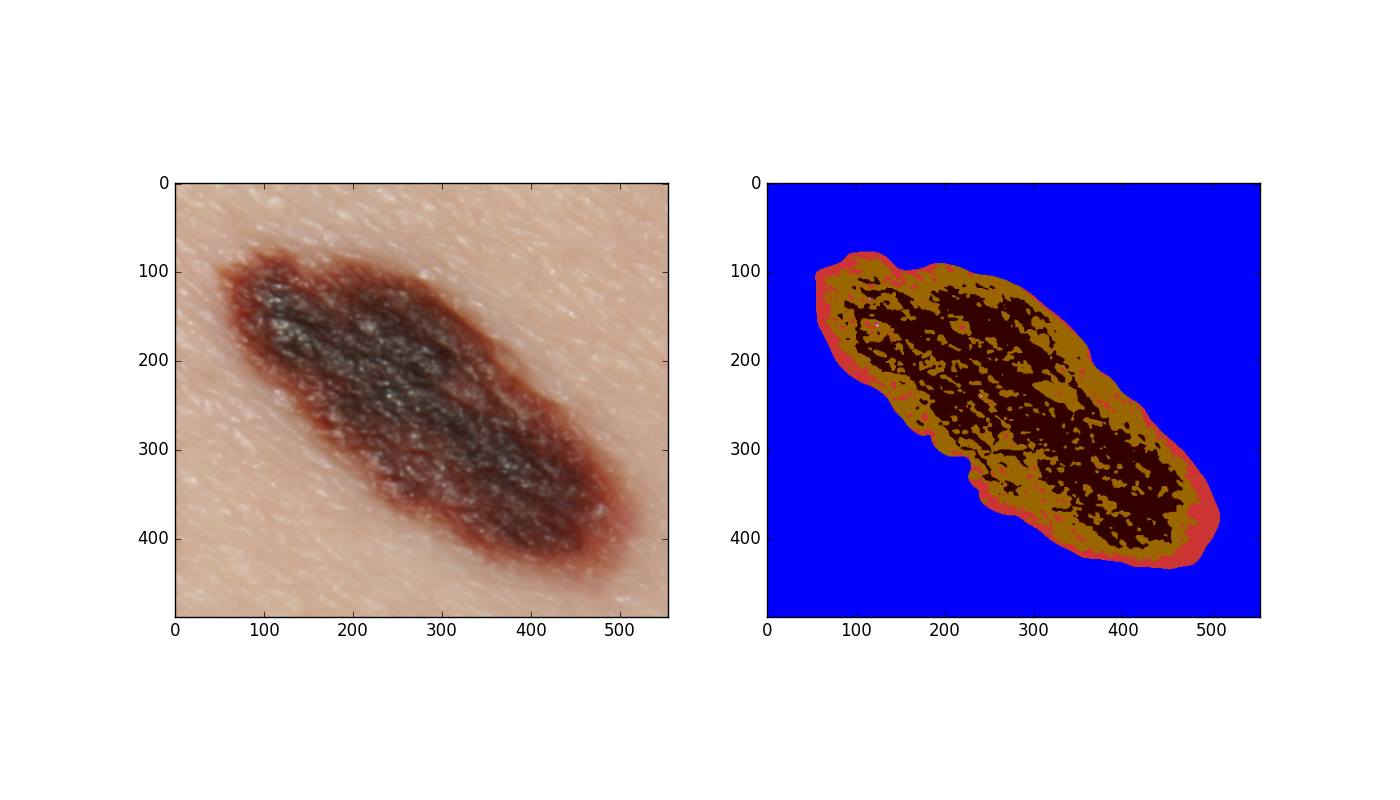
\includegraphics[height=8cm,keepaspectratio]{assets/color/examples/color_3.png}
    \caption{Example of color score 3}
    \label{fig:color_3}
\end{figure}
\begin{figure}[H]
    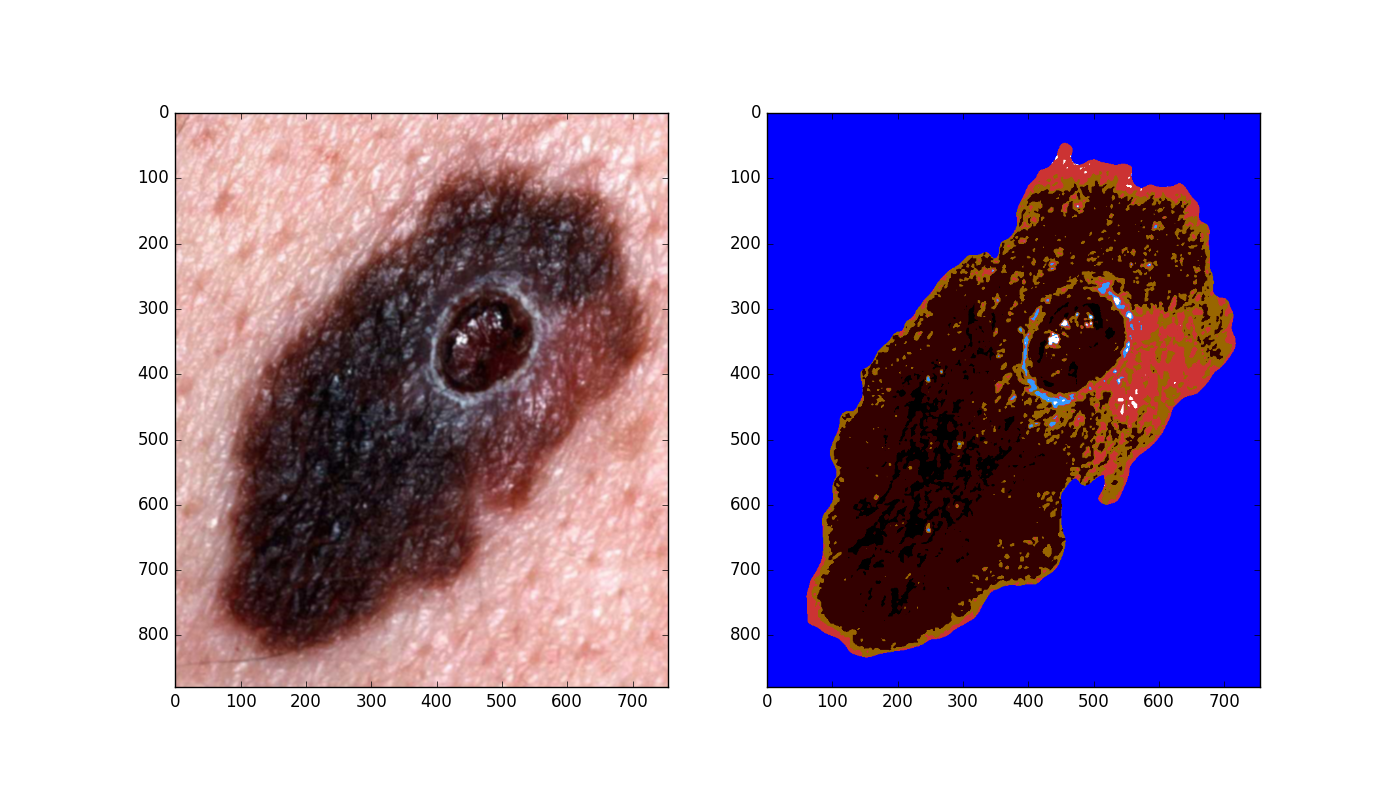
\includegraphics[height=8cm,keepaspectratio]{assets/color/examples/color_4.png}
    \caption{Example of color score 4}
    \label{fig:color_4}
\end{figure}